%-------------------------------------------------------------------------
% Design Project Input/Output Module Description
%-------------------------------------------------------------------------

\clearpage
\section{Force Input Module}
\label{sec-input-force}

This input module enables your IoT device to sense the amount of force
exerted on the surface of a squeeze pad. The sensor is a resistor with a
resistance that varies depending on how much force is exerted on the
squeeze pad (e.g., by squeezing it between two fingers); the resistance
is high (infinite) when there is no force and low when the force is
high. The Arduino cannot directly sense resistance, but we can set up a
voltage divider so that the Arduino can sense voltage instead. This way,
as we apply more force to the sensor, the voltage the Arduino reads
decreases.

% FIXME: replace 'ohm' with symbol..

A sample circuit and Arduino code is shown below to get you started.
The voltage divider circuit is formed by the force sensor and the
\wu{10}{kohm} resistor, and the Arduino reads the voltage from one end
of the resistor to ground. The example code will print the analog
reading from the force sensor on the serial monitor, similar to how we
printed the analog reading from the grayscale sensor in Lab~2. After
setting up the circuit and programming the Arduino, open the serial
monitor and check the value the force sensor is detecting. Then try
squeezing the squeeze pad between two fingers and see the reading
increase.

\vspace{0.1in}
\begin{minipage}[t]{0.49\tw}
  \vspace{0pt}

  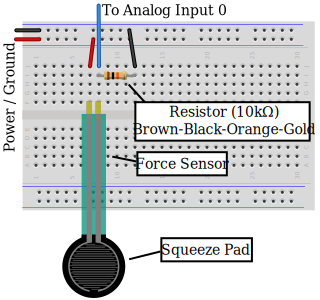
\includegraphics[width=\tw]{input-force-annotated.svg.pdf}
\end{minipage}
\hfill
\begin{minipage}[t]{0.49\tw}
  \vspace{0.1in}
  \begin{Verbatim}[gobble=3,fontsize=\small]
    int pin_force = 0;

    void setup() {
      Serial.begin(9600);
      pinMode( pin_force, INPUT );
    }

    void loop() {
      int force = analogRead( pin_force );

      Serial.println( force );
      delay(1000);
    }
  \end{Verbatim}
\end{minipage}
\vspace{0.1in}

%Questions:
